\documentclass{article}

\usepackage[colorlinks, urlcolor=blue, linkcolor=red, citecolor=green]{hyperref}
\usepackage{fancyhdr} %设置页眉和页脚的
\usepackage{extramarks} %设置continue那玩意的
\usepackage{amsmath}
\usepackage{amsthm}
\usepackage{amsfonts}
\usepackage{tikz} %画线的
\usepackage[plain]{algorithm}
\usepackage{algpseudocode}
\usepackage{enumerate}

\usetikzlibrary{automata,positioning}

%表
\usepackage{booktabs}
\usepackage{multirow}
\usepackage{array}
\usepackage{caption}
\DeclareCaptionFont{heiti}{\heiti} %还可以定义其他的
\captionsetup{labelsep=space, font={small, bf}, skip=2pt} %space可以改成quad

%图
%*****************图片及其相关设置***************************
\usepackage{graphicx}
\graphicspath{{tupian/}}
\usepackage{subfigure}
% 导入tikz包
\usepackage{tikz}
\usetikzlibrary{math}

%*****************代码相关设置***************************
\usepackage{pythonhighlight}
\usepackage{listings}
\lstset{language=R,
    basicstyle=\small\ttfamily,
    otherkeywords={0,1,2,3,4,5,6,7,8,9},
    morekeywords={TRUE,FALSE},
    deletekeywords={data,frame,length,as,character},
    keywordstyle=\color{blue},
    backgroundcolor=\color[RGB]{245,245,244},
}
%
% Basic Document Settings
%

\topmargin=-0.45in
\evensidemargin=0in
\oddsidemargin=0in
\textwidth=6.5in
\textheight=9.0in
\headsep=0.25in

\linespread{1.1}

\pagestyle{fancy}
\lhead{\hmwkAuthorName}
\chead{\hmwkClass}
\rhead{\firstxmark}
\lfoot{\lastxmark}
\cfoot{\thepage}

\renewcommand\headrulewidth{0.4pt}
\renewcommand\footrulewidth{0.4pt}

\setlength\parindent{0pt}

%
% Create Problem Sections
%

\newcommand{\enterProblemHeader}[1]{
    \nobreak\extramarks{}{Project \arabic{#1} continued on next page\ldots}\nobreak{}
    \nobreak\extramarks{Project \arabic{#1} (continued)}{Project \arabic{#1} continued on next page\ldots}\nobreak{}
}

\newcommand{\exitProblemHeader}[1]{
    \nobreak\extramarks{Project \arabic{#1} (continued)}{Project \arabic{#1} continued on next page\ldots}\nobreak{}
    \stepcounter{#1}
    \nobreak\extramarks{Project \arabic{#1}}{}\nobreak{}
}

%\setcounter{secnumdepth}{0}
\newcounter{partCounter}
\newcounter{homeworkProblemCounter}
\setcounter{homeworkProblemCounter}{1}
\nobreak\extramarks{Project \arabic{homeworkProblemCounter}}{}\nobreak{}

\newenvironment{homeworkProblem}{
    \section{Project \arabic{homeworkProblemCounter}}
    \setcounter{partCounter}{1}
    \enterProblemHeader{homeworkProblemCounter}
}{
    \exitProblemHeader{homeworkProblemCounter}
}

%
% Homework Details
%   - Title
%   - Due date
%   - Class
%   - Section/Time
%   - Instructor
%   - Author
%

\newcommand{\hmwkTitle}{Project 1}
\newcommand{\hmwkDueDate}{Aprl 11, 2021}
\newcommand{\hmwkClass}{Time Series Analysis}
\newcommand{\hmwkClassTime}{}
\newcommand{\hmwkClassInstructor}{Professor Tianwei Yu}
\newcommand{\hmwkAuthorName}{Peng Deng}
\newcommand{\hmwkAuthorSchool}{School of Data Science}
\newcommand{\hmwkAuthorNumber}{Sno.220041042}
%
% Title Page
%

\title{
    \vspace{2in}
    \textmd{\textbf{\hmwkClass: \hmwkTitle}}\\
    \normalsize\vspace{0.1in}\small{Due\ on\ \hmwkDueDate}\\
    \vspace{0.1in}\large{\textit{\hmwkClassInstructor\ \hmwkClassTime}}
    \vspace{3in}
}

\author{\textbf{\hmwkAuthorName}}


\date{}

\renewcommand{\part}[1]{\textbf{\large Part \Alph{partCounter}}\stepcounter{partCounter}\\}

%
% Various Helper Commands
%

% Useful for algorithms
\newcommand{\alg}[1]{\textsc{\bfseries \footnotesize #1}}
\usepackage[algo2e,vlined,ruled]{algorithm2e}

% For derivatives
\newcommand{\deriv}[1]{\frac{\mathrm{d}}{\mathrm{d}x} (#1)}

% For partial derivatives
\newcommand{\pderiv}[2]{\frac{\partial}{\partial #1} (#2)}

% Integral dx
\newcommand{\dx}{\mathrm{d}x}

% Alias for the Solution section header
\newcommand{\solution}{\textbf{\large Solution}}

% Probability commands: Expectation, Variance, Covariance, Bias
\newcommand{\E}{\mathrm{E}}
\newcommand{\Var}{\mathrm{Var}}
\newcommand{\Cov}{\mathrm{Cov}}
\newcommand{\Bias}{\mathrm{Bias}}
\begin{document}

\maketitle
\thispagestyle{empty}
\pagebreak
\thispagestyle{empty}
\tableofcontents

\newpage
\setcounter{page}{1}
\section{Problem statement}
Use dataset “chicagoNMMAPS” from the “dlnm” package in R. The data set contains daily mortality, weather, and pollution data for Chicago from 1987 to 2000. 
We would like to use the data to do some training and forecast by implementing some timeseries models.
\vspace{4pt}
\section{Dataset overview}

Firstly, we can have a quick look at the dataset, the meanings of the headers in the dataset are explained as follow:

    \quad - date: Date in the period 1987-2000

    \quad - time: The sequence of observations

    \quad - year: Year

    \quad - month: Month (numeric)

    \quad - doy: Day of the year

    \quad - dow: Day of the week (factor)

    \quad - death: Counts of all cause mortality excluding accident

    \quad - cvd: Cardiovascular Deaths

    \quad - resp: Respiratory Deaths

    \quad - temp: Mean temperature (in Celsius degrees)

    \quad - dptp: Dew point temperature

    \quad - rhum: Mean relative humidity

    \quad - pm10: PM10

    \quad - o3: Ozone

\vspace{4pt}
\section{Data preprocessing}

First, combine the daily data into monthly data. For data with missing values, such as daily PM10, replace the NA with average over non-NA values over the month before taking monthly average. We can see that this preprocessing equals to just take average on non-NA values. So our preprocessing is just to take 
average on non-NA values in every month and separate the data into three segments:
    
    \quad - Training: 1987.1-1995.12

    \quad - Validation: 1996.1-1997.12

    \quad - Testing: 1998.1-2000.12

\vspace{4pt}
\section{Univariate analysis of the cardiovascular death(cvd)}
\subsection{STL and EST model}

We know that stl (Seasonal and Trend decomposition using Loess) is a very useful tool to decompose data. Firstly, we just use the following parameters of stl 
to do a decomposition of the training dataset.
\begin{lstlisting}[language=R]
cvd.stl = stl(cvd.ts.training, s.window=4, t.window=12, robust=TRUE)
\end{lstlisting}

\begin{figure}[H]
    \centering
    \subfigure[The decomposition result by stl]{\label{stl1}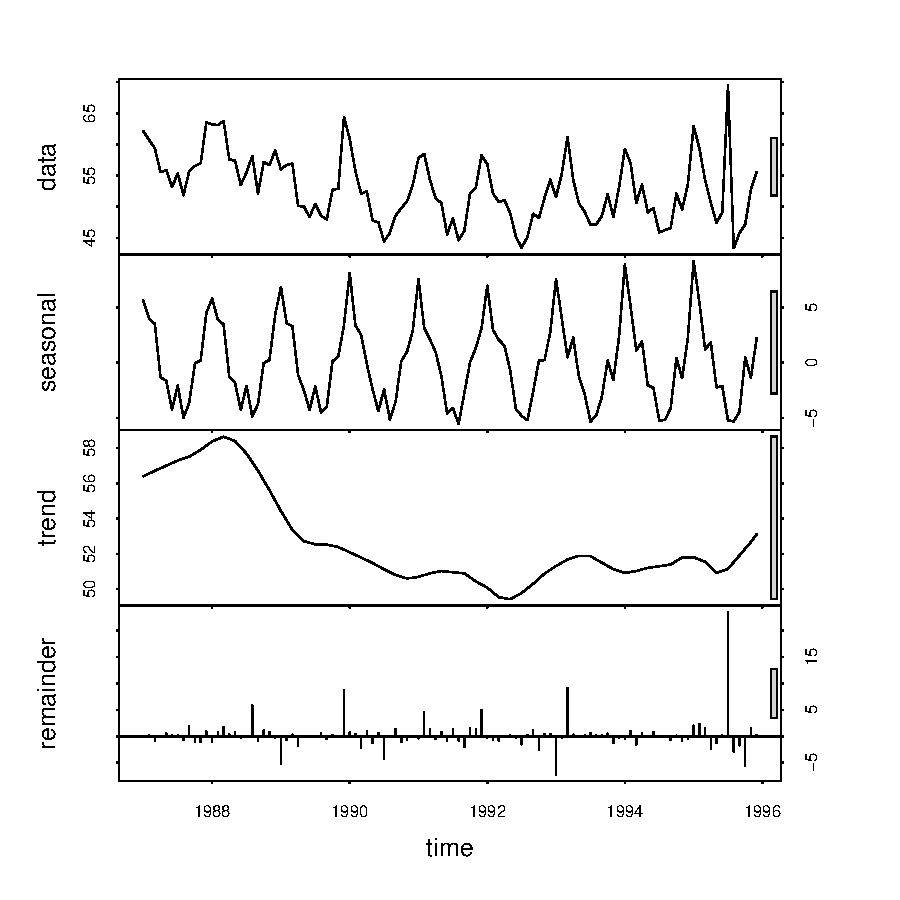
\includegraphics[width=0.4\linewidth]{images/cvd-stl-decom}}
    \quad
    \subfigure[Holt-Winters filtering]{\label{stl2}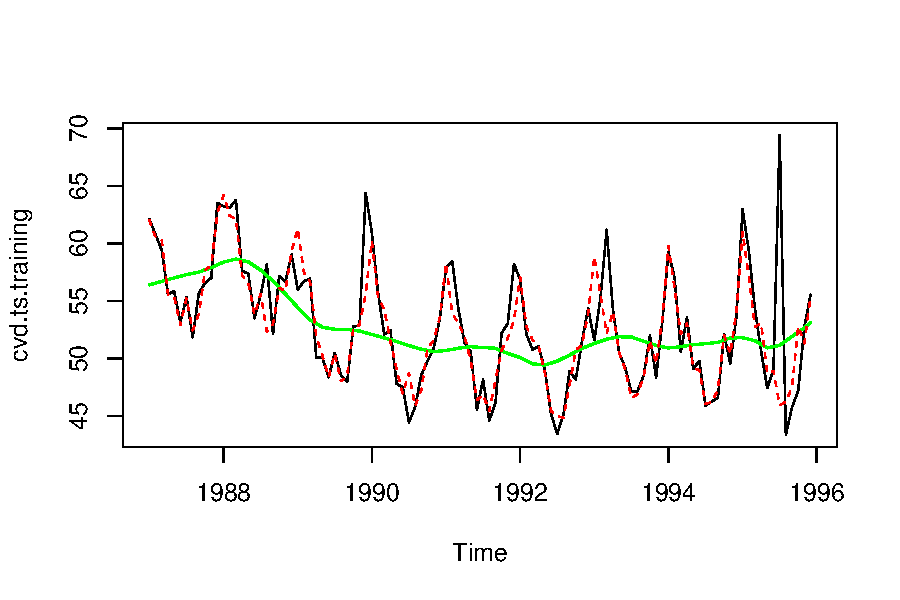
\includegraphics[width=0.5\linewidth]{images/cvd-stl-fit}}
    \caption{stl decomposition and fitted figure}
    \label{stl}
\end{figure}

Then, we can have a quik look of the decomposition result as Figure \ref{stl}. In Figure \ref{stl2}, the black line is the original training data, the green line is the trend, and the red dashed line is the fitted value.


In order to see if the decomposition is good, we can plot the acf of the decomposition remainder as Figure \ref{stl-acf}. As we can see in Figure \ref{stl-acf}, there is a little acf, so that it is not suitable to do forecast just use stl. 
Thus, we implement ETS as an complement to do forecast. 
\begin{figure}[htbp]
    \centering
    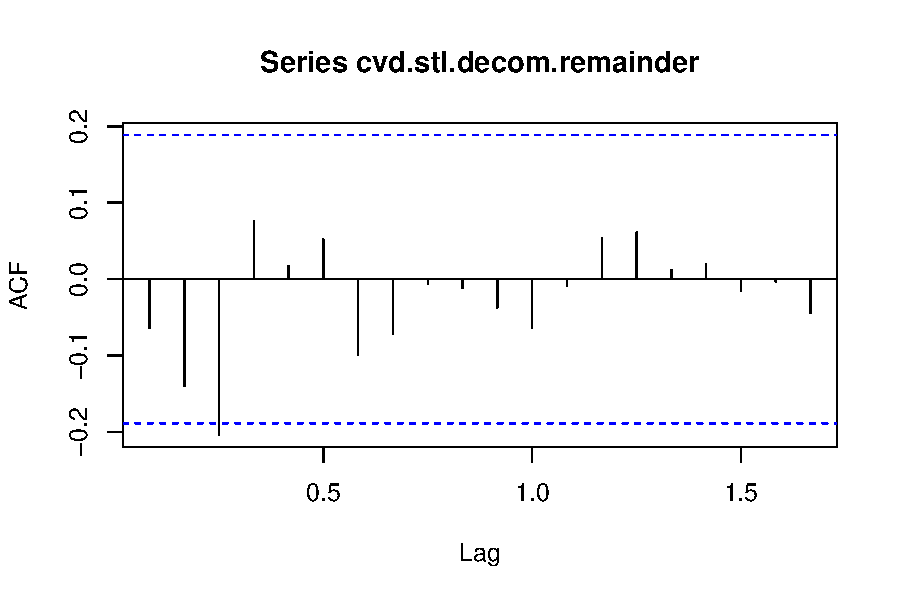
\includegraphics[width=0.58\linewidth]{images/cvd-stl-acf}
    \caption{The ACF of residuals}
    \label{stl-acf}
\end{figure}

\begin{figure}[htbp]
    \centering
    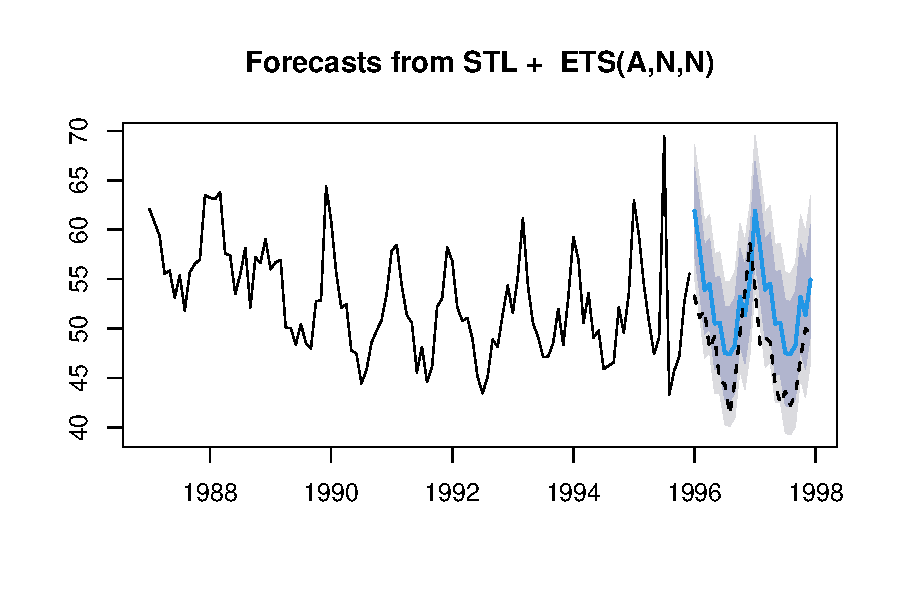
\includegraphics[width=0.6\linewidth]{images/cvs-stl-forecast}
    \caption{The prediction on validation dataset with STL and ETS}
    \label{stl-forecast}
\end{figure}

The forecast result is showed as Figure \ref{stl-forecast}. As we can see in Figure \ref{stl-forecast}, the dashed line is the true 
value of validation dataset, the blue line is the forcasted value of Validation dataset. Then, we calculated the Root Mean Squard Error (RMSE) on the validation dataset. 

$\star$ RMSE = 5.61 $\star$

\vspace{4pt}
\subsection{Holt-Winters model}

As we know that there are holt-winters models with additive seasonal component and with multiplicative seasonal component. 
As we can see, there is no evident multiplicative seasonal component in the time series, so we just use the holt-winters model 
with additive seasonal component. The fitted figures are as Figure \ref{hw}.

\begin{figure}[H]
    \centering
    \subfigure[Holt-Winters decomposition]{\label{hw1}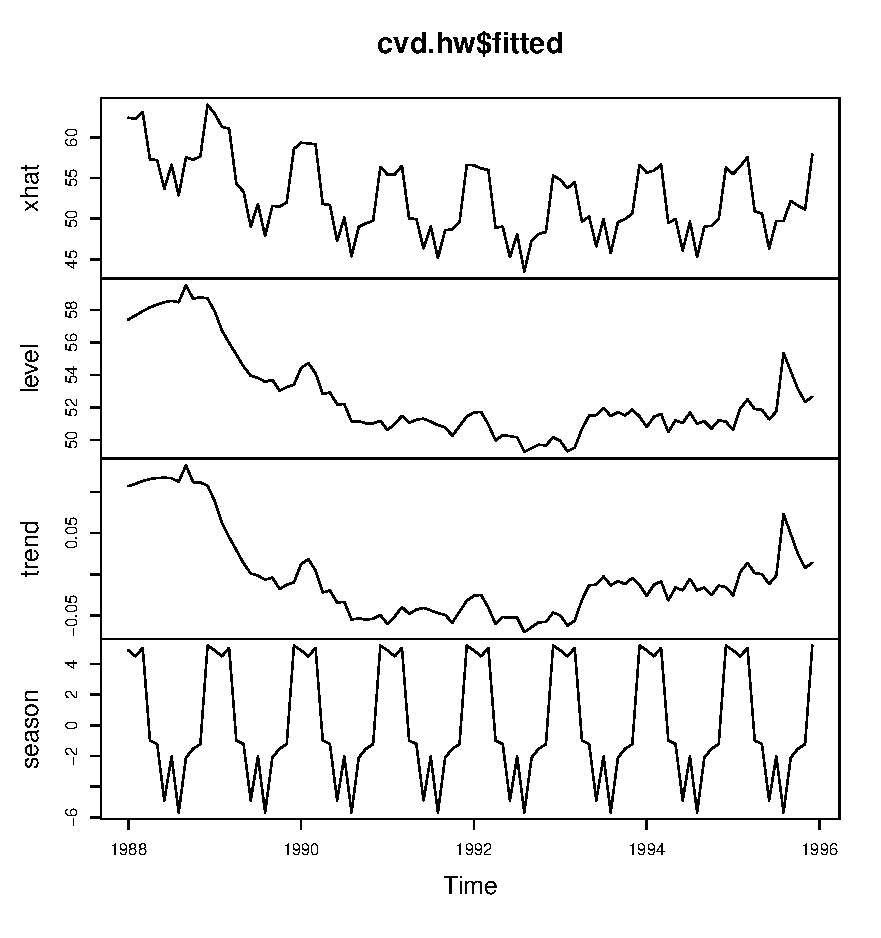
\includegraphics[width=0.4\linewidth]{images/cvd-hw-fit1}}
    \quad
    \subfigure[Holt-Winters filtering]{\label{hw2}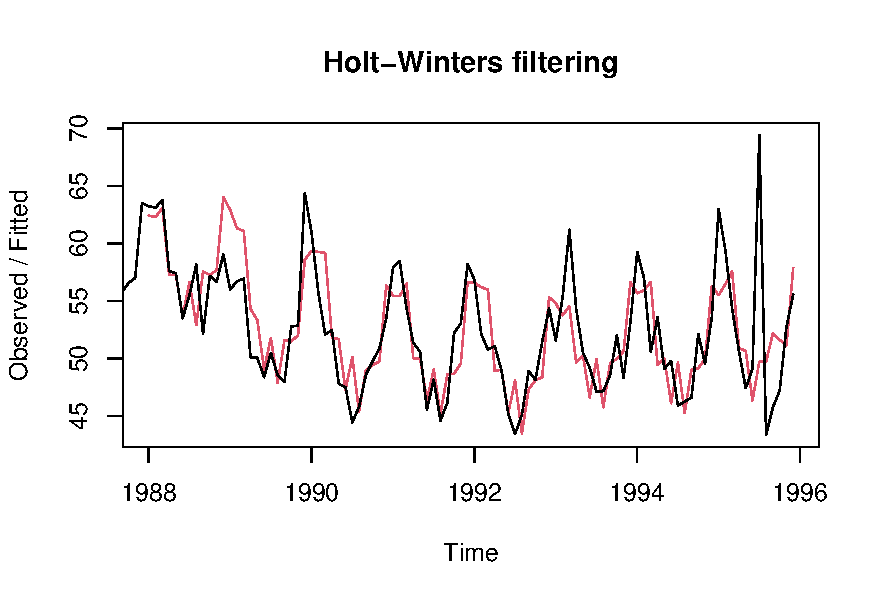
\includegraphics[width=0.55\linewidth]{images/cvd-hw-fit2}}
    \caption{Holt-winters model fitted figure}
    \label{hw}
\end{figure}
Then, we plot the ACF figure of the residuals according to the model result as Figure \ref{acf1}. As we can see, There is no significant auto-correlation in the residuals, which means our model is 
somehow good to fit the data.
\begin{figure}[htbp]
    \centering
    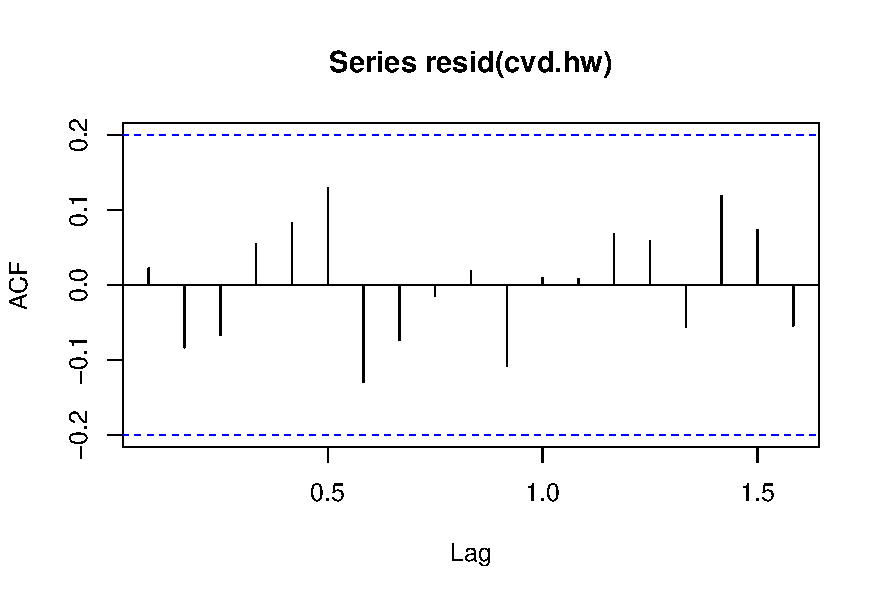
\includegraphics[width=0.65\linewidth]{images/cvd-hw-res-acf}
    \caption{The ACF of residuals}
    \label{acf1}
\end{figure}

Then, we would like to implement the fitted model on the validation dataset(1996.1-1997.12) in order to test the model's prediction accuracy. As we can see in Figure \ref{val}, the dashed line is the true 
value of validation dataset, the blue line is the forcasted value of validation dataset. Then, we calculated the Root Mean Squard Error (RMSE) on the validation dataset. 

$\star$ RMSE = 5.08 $\star$
\begin{figure}[H]
    \centering
    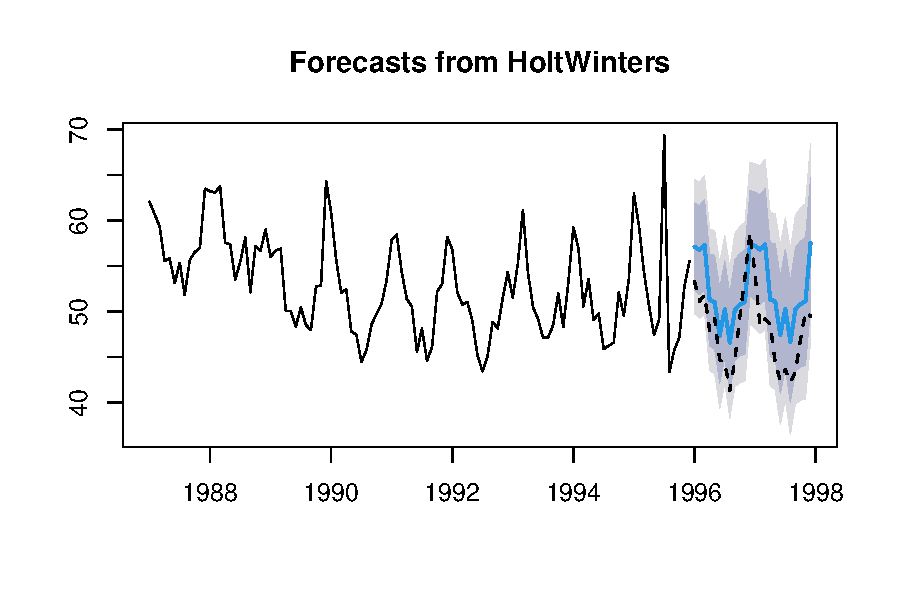
\includegraphics[width=0.65\linewidth]{images/cvd-hw-val}
    \caption{The prediction on validation dataset with holt-winters model}
    \label{val}
\end{figure}

\vspace{4pt}
\subsection{Seasonal ARIMA model}

As we can see, there is evident seasonal component, so that we would like to use Seasonal ARIMA instead of just ARIMA. In order to determine the parameters in seasonal ARIMA, we call "auto.arima" in R as follow. 
\begin{lstlisting}
cvd.arima = auto.arima(cvd.ts.training)
\end{lstlisting}
Then, we get the parameters of Seasonal ARIMA is:
ARIMA(1,1,1)(0,0,2)[12]. The fitted figures are as Figure \ref{arima-fit}.
\begin{figure}[H]
    \centering
    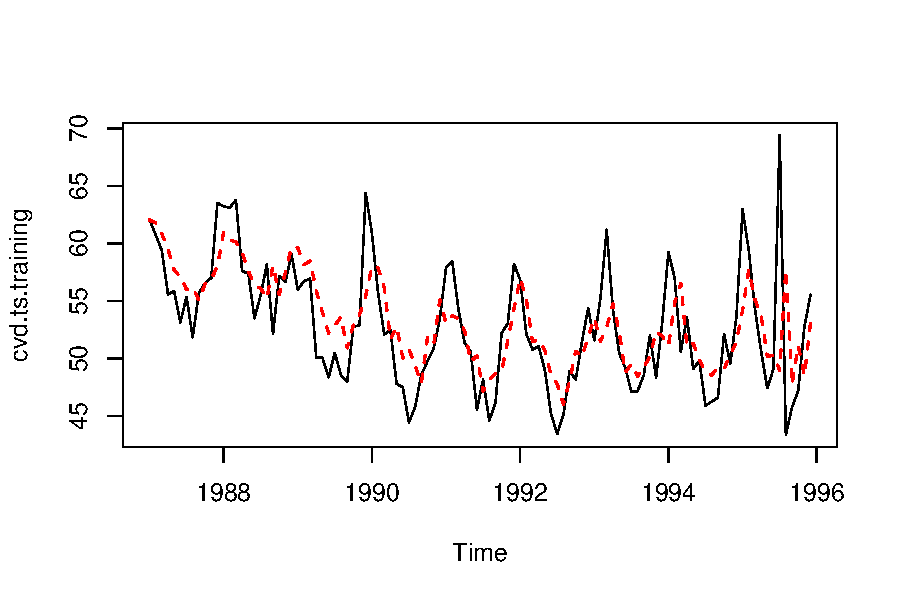
\includegraphics[width=0.65\linewidth]{images/cvd-arima-fit}
    \caption{Seasonal ARIMA model fitted figure}
    \label{arima-fit}
\end{figure}
Then, we plot the residuals and the ACF figure of the residuals according to the Seasonal ARIMA model result as Figure \ref{arima}, which means we are going to check residuals.
\begin{figure}[H]
    \centering
    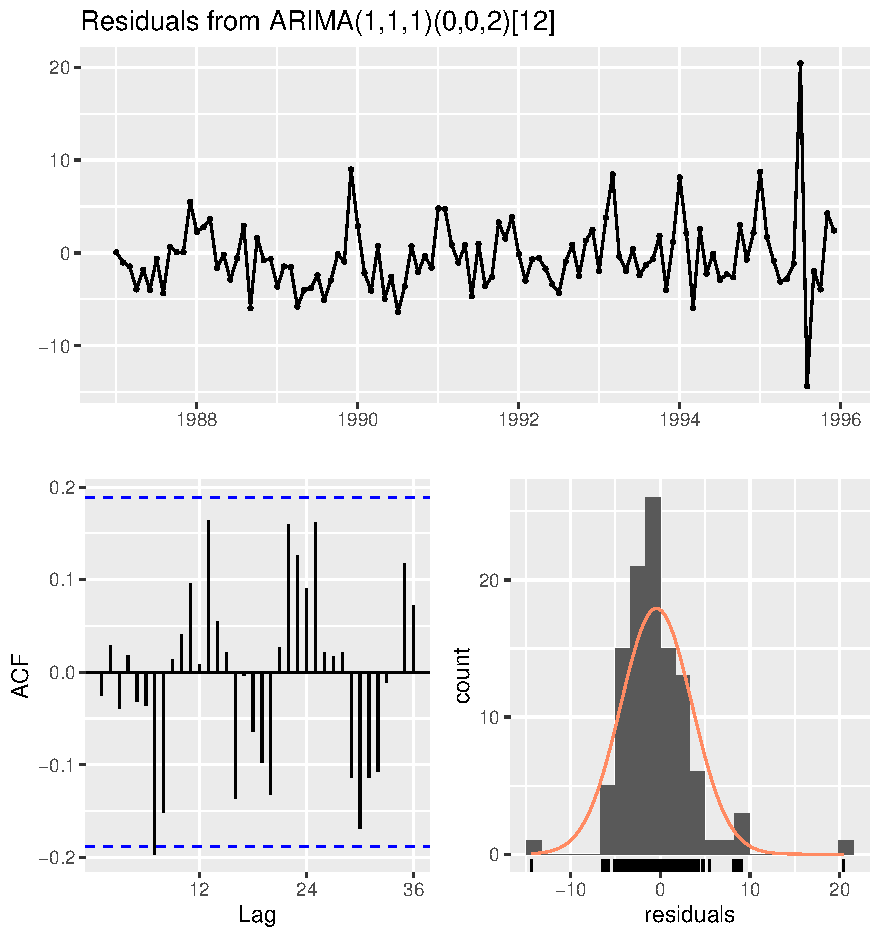
\includegraphics[width=0.65\linewidth]{images/cvd-arima-check}
    \caption{Check residuals of Seasonal ARIMA}
    \label{arima}
\end{figure}



As we can see from Figure \ref{arima}, there is significant acf, so that the model is not very good. However, we can do the Ljung-Box test of the residuals to see if the residuals exhibit serial correlation, the result is as follow:
\begin{lstlisting}
            Ljung-Box test

    data:  Residuals from ARIMA(1,1,1)(0,0,2)[12]
    Q* = 23.289, df = 18, p-value = 0.1797
    
    Model df: 4.   Total lags used: 22
\end{lstlisting}
As we can see from the Ljung-Box test, the p-value equals 0.1797, which is larger than 0.05, so that we should not reject the null hypothesis, which means 
the residuals does not exhibit serial correlation. Thus, we can believe that the Seasonal ARIMA model is suitable.

Then, we would like to implement the fitted Seasonal ARIMA model on the validation dataset(1996.1-1997.12) in order to test the model's prediction accuracy. As we can see in Figure \ref{cvd-arima-forecast}, the dashed line is the true 
value of validation dataset, the blue line is the forcasted value of Validation dataset. Then, we calculated the Root Mean Squard Error (RMSE) on the validation dataset. 

$\star$ RMSE = 6.35 $\star$
\begin{figure}[H]
    \centering
    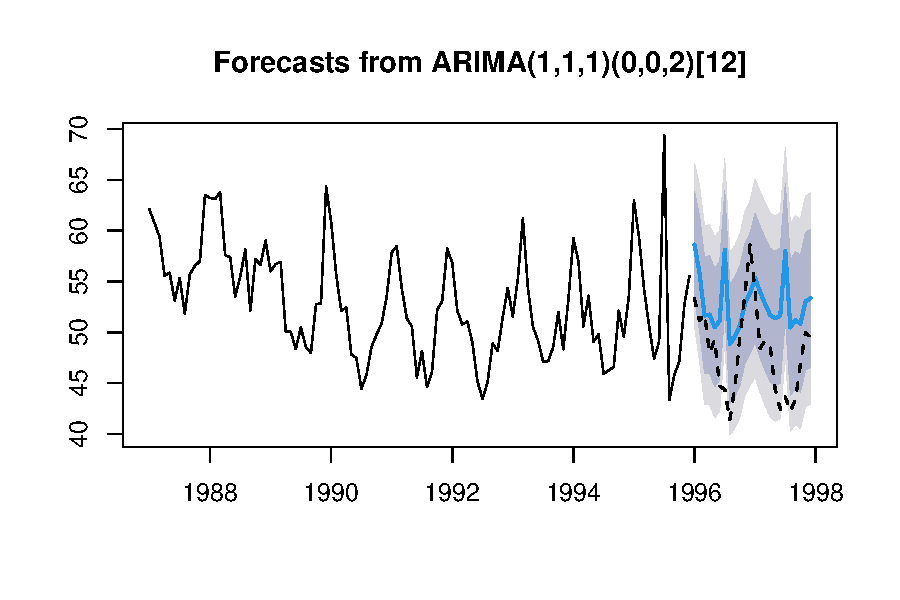
\includegraphics[width=0.65\linewidth]{images/cvd-arima-forecast}
    \caption{The prediction on validation dataset with Seasonal ARIMA model}
    \label{cvd-arima-forecast}
\end{figure}

\vspace{4pt}
\subsection{Run the best model}

According to the RMSE value of the three models as follow, we can find that the \textbf{holt-winters model} is the bset. Thus, we would like to run holt-winters in the following.

\quad - STL+ETS:  RMSE = 5.61

\quad - Holt-winters:  RMSE = 5.08 $\star$

\quad - Seasonal ARIMA:  RMSE = 6.35 

Firstly, we would like to run the best-performing model (holt-winters) on the 1987.1-1997.12 data (training dataset and validation dataset). 
We just use the holt-winters model 
with additive seasonal component. The fitted figures are as Figure \ref{best-fit}.
\begin{figure}[H]
    \centering
    \subfigure[Holt-Winters decomposition]{\label{best-hw1}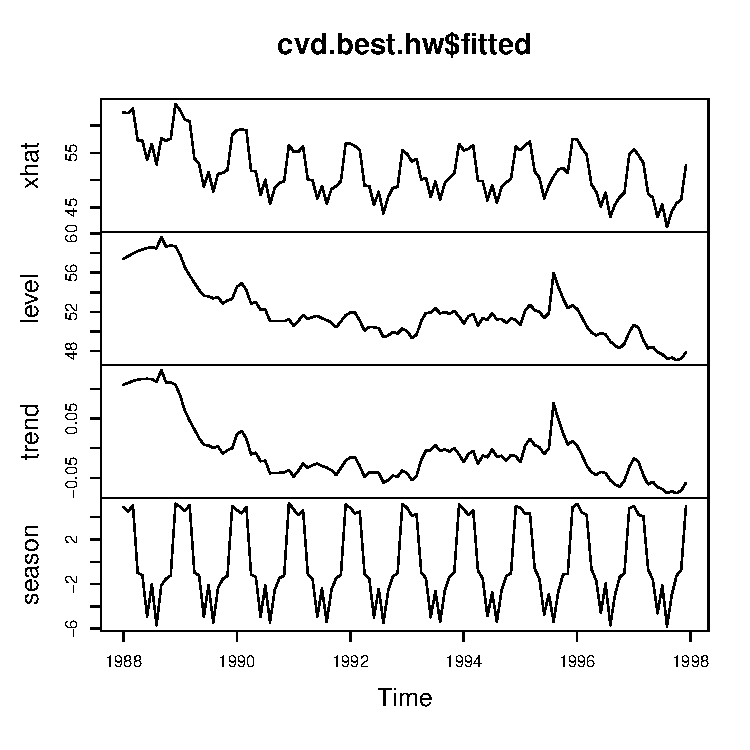
\includegraphics[width=0.4\linewidth]{images/best-fit1}}
    \quad
    \subfigure[Holt-Winters filtering]{\label{best-hw2}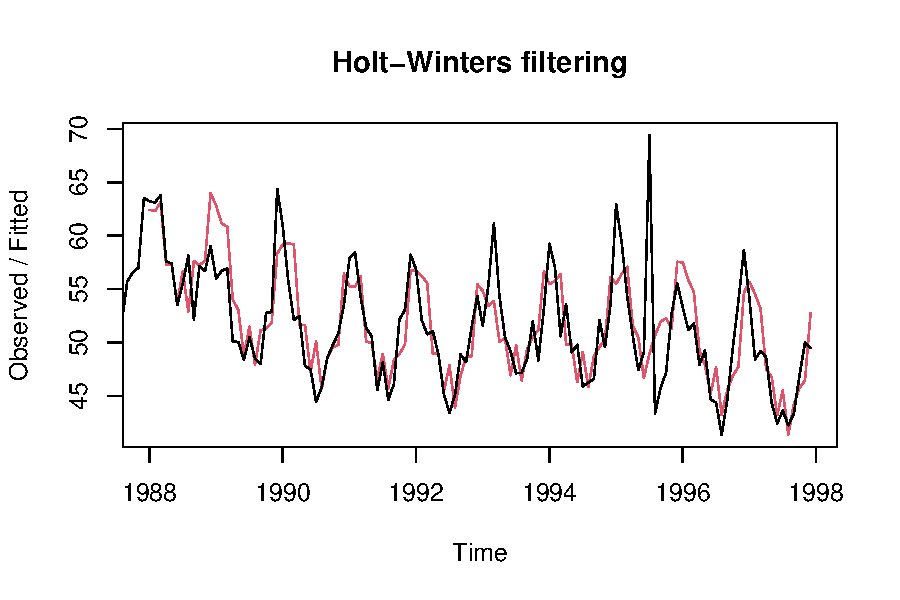
\includegraphics[width=0.55\linewidth]{images/best-fit2}}
    \caption{Best model fitted figure}
    \label{best-fit}
\end{figure}
Then, we plot the ACF figure of the residuals according to the model result as Figure \ref{best-acf}. 
\begin{figure}[H]
    \centering
    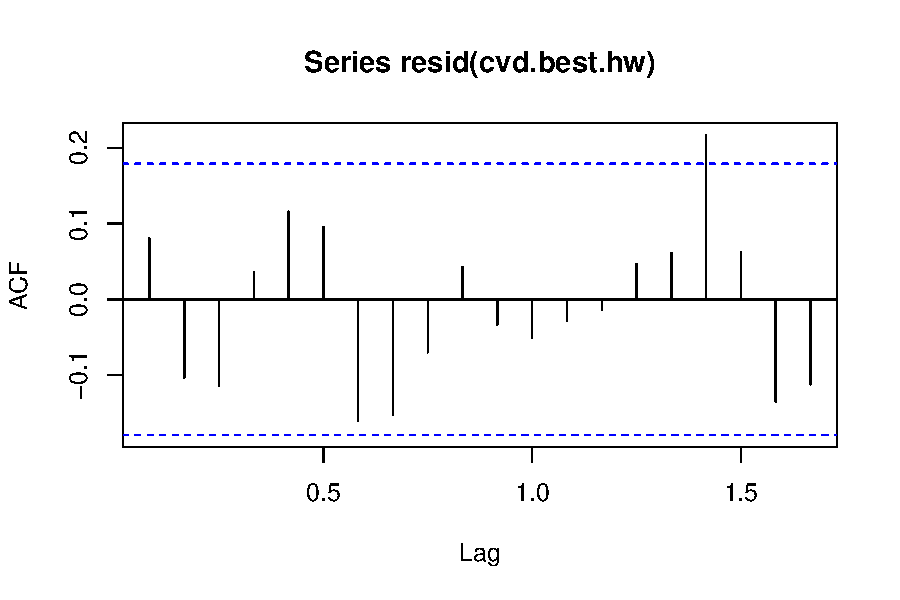
\includegraphics[width=0.65\linewidth]{images/best-acf}
    \caption{The ACF of residuals with the best model}
    \label{best-acf}
\end{figure}
As we can see from Figure \ref{best-acf}, 
there is evident acf. Thus, we have to do Ljung-Box test of the residuals to see if the residuals exhibit serial correlation, the result is as follow:
\begin{lstlisting}
    
	    Box-Ljung test

    data:  resid(cvd.best.hw)
    X-squared = 0.79242, df = 1, p-value = 0.3734
\end{lstlisting}
As we can see from the Ljung-Box test, the p-value equals 0.3734, which is larger than 0.05, so that we should not reject the null hypothesis, which means 
the residuals does not exhibit serial correlation. Thus, we can believe that the best model (holt-winters) is suitable.

\vspace{4pt}
Then, we would like to implement the fitted model on the test dataset(1998.1-2000.12) in order to do forecast. As we can see in Figure \ref{best-forecast}, the dashed line is the true 
value of test dataset, the blue line is the forcasted value of test dataset. 
\begin{figure}[H]
    \centering
    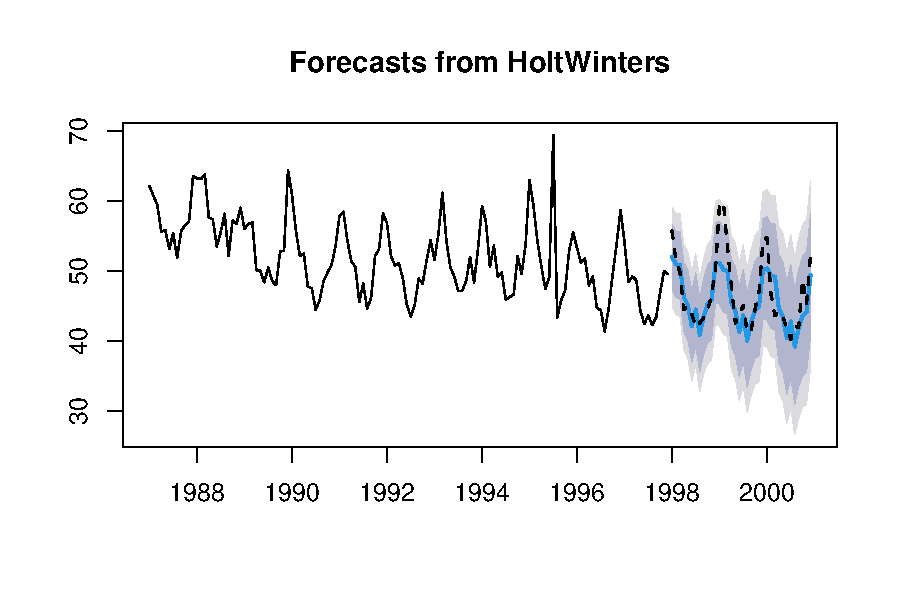
\includegraphics[width=0.65\linewidth]{images/best-forecast}
    \caption{The prediction on test dataset with best model (holt-winters)}
    \label{best-forecast}
\end{figure}
Then, we calculated the Root Mean Squard Error (RMSE) on the test dataset. 

$\star$ RMSE = 3.16 $\star$

We can see that the forecast is pretty good, it is very near to the true value. Besides, the RSME equals 3.16, which is relatively small.
\vspace{4pt}

Above all, we can conclude that the holt-winters model performs very good.

\vspace{4pt}
\section{Multivariate analysis of the cardiovascular death(cvd)}   

Now consider also the temperature (temp) and the pollution variables (PM10 and o3), which could help predict mortality of some diseases. Use the cardiovascular death as outcome as well.

\vspace{4pt}
\subsection{ARIMA with external variables}

Firsly, lets have a quik look of the value of the four variables (cvd, temp, pm10 and o3). their value on training data set is showed as Figure \ref{data-all}.

\vspace{-10pt}
\begin{figure}[H]
    \centering
    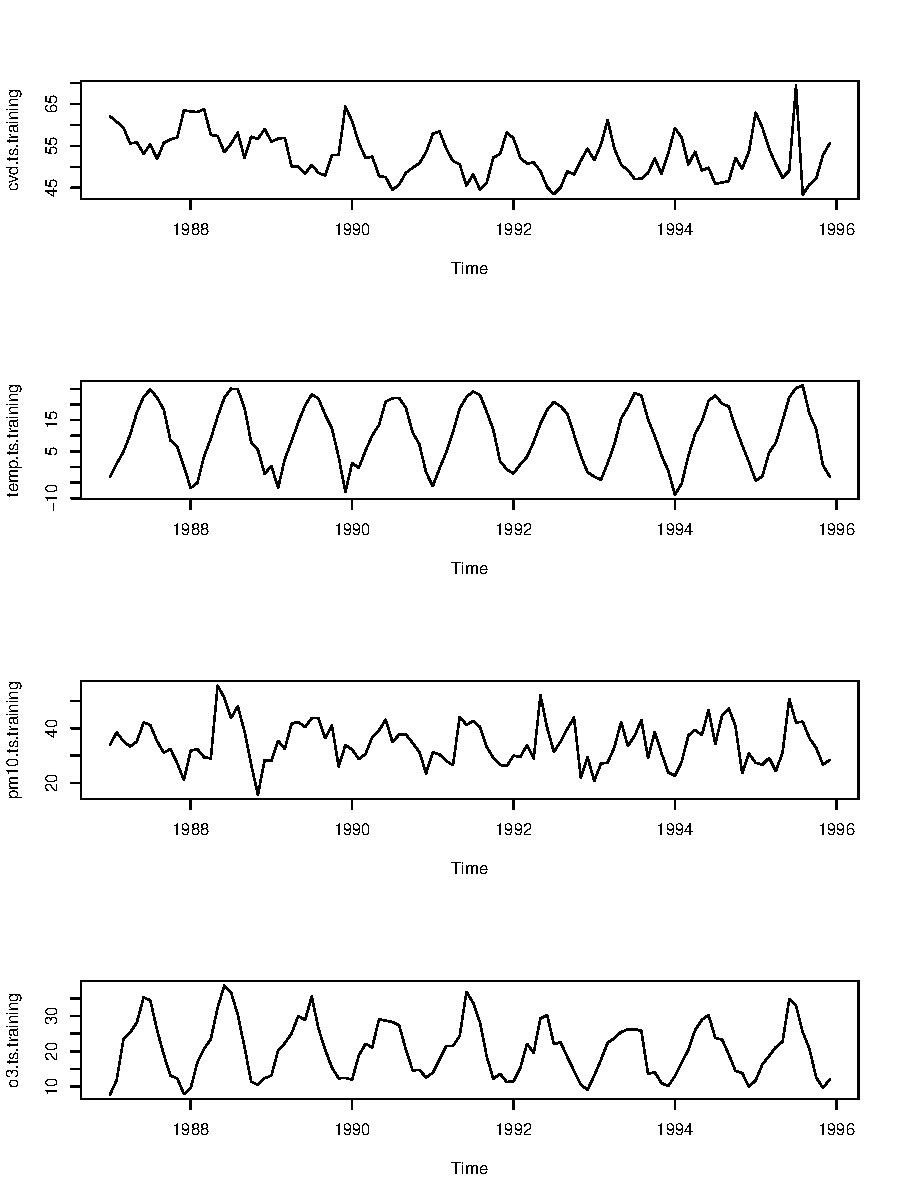
\includegraphics[width=0.55\linewidth]{images/multi}
    \caption{The value of four variables on training dataset}
    \label{data-all}
\end{figure}
As we can see from Figure \ref{data-all}, there may have some relationships between cvd and external variables. Then, we implement auto.arima to choose the parameters of 
"ARIMA with external variables" model.
\begin{lstlisting}
multi.arima.external = auto.arima(cvd.ts.training, 
            xreg=cbind(temp.ts.training, pm10.ts.training, o3.ts.training))
\end{lstlisting}
Then, we can see the result as follow
\begin{lstlisting}
Series: cvd.ts.training 
Regression with ARIMA(0,1,1) errors 

Coefficients:
        ma1  temp.ts.training  pm10.ts.training  o3.ts.training
    -0.8198           -0.4280            0.0409          0.1229
s.e.  0.0602           0.0533            0.0634          0.0709

sigma^2 estimated as 12.57:  log likelihood=-285.76
AIC=581.52   AICc=582.11   BIC=594.88
\end{lstlisting}
Thus, we get the parameters of ARIMA with external variables is:
the error $\eta_t$ is ARIMA(0,1,1). The fitted figure is as Figure \ref{arima-external-fit}.

\vspace{-15pt}
\begin{figure}[H]
    \centering
    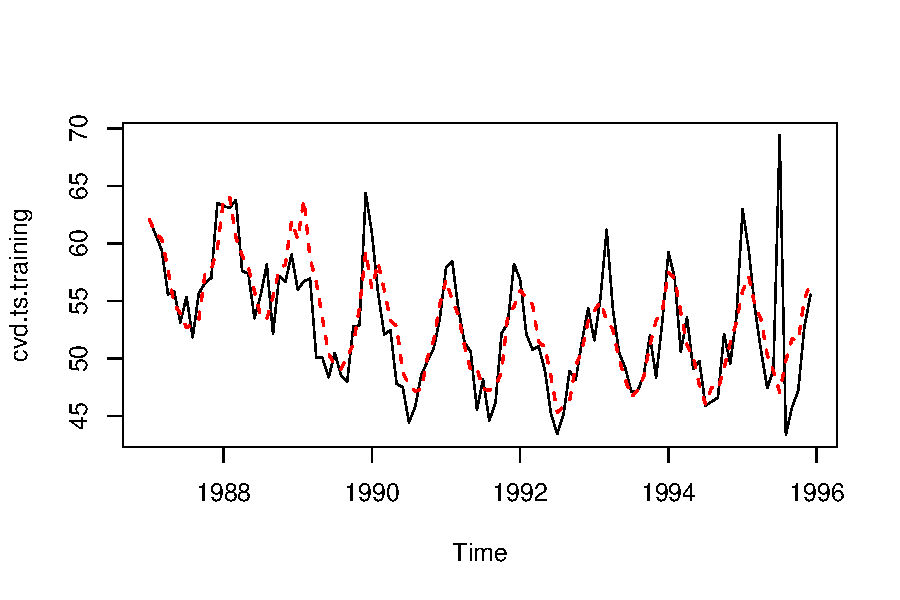
\includegraphics[width=0.6\linewidth]{images/arima-external-fit}
    \caption{ARIMA with external variables model fitted figure}
    \label{arima-external-fit}
\end{figure}
Then, we plot the residuals and the ACF figure of the residuals according to the the model result as Figure \ref{arima-external-acf}, which means we are going to check residuals. 
\begin{figure}[H]
    \centering
    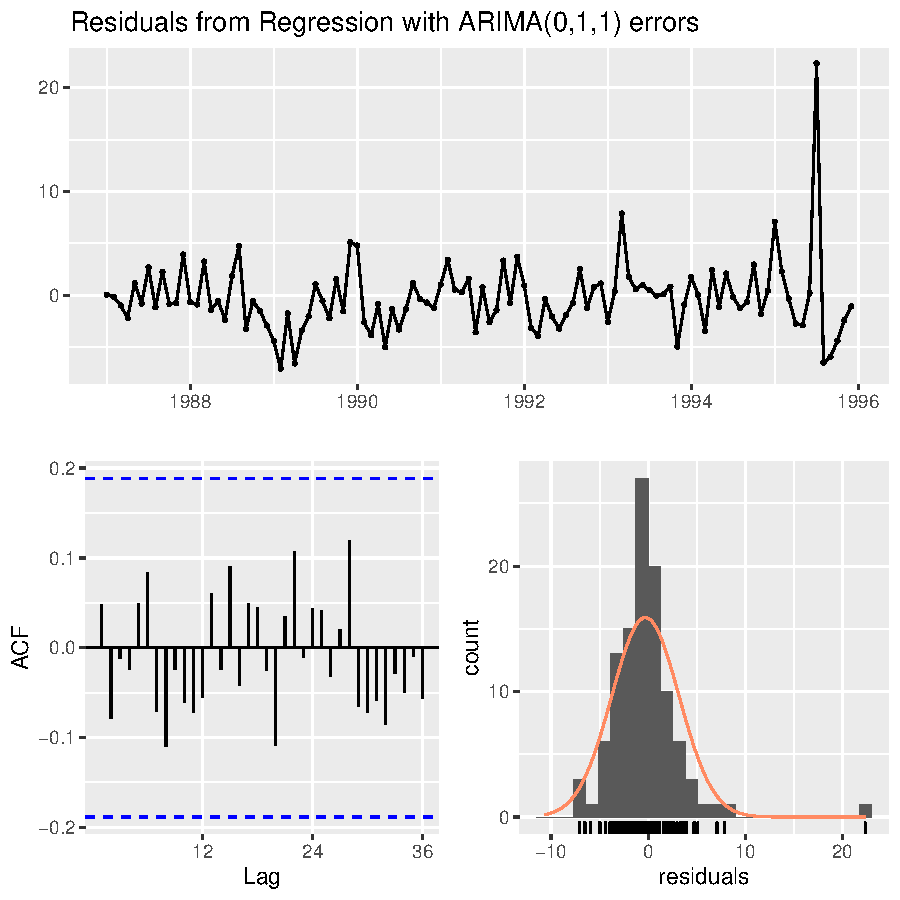
\includegraphics[width=0.58\linewidth]{images/arima-external-acf}
    \caption{Check residuals of ARIMA with external variables}
    \label{arima-external-acf}
\end{figure}
As we can see from Figure \ref{arima-external-acf}, there is no significant acf, so that the model is somehow very good. 

\vspace{4pt}
Then, we would like to implement the fitted ARIMA with external variables model on the validation dataset(1996.1-1997.12) in order to test the model's prediction accuracy. As we can see in Figure \ref{arima-external-val}, the dashed line is the true 
value of validation dataset, the blue line is the forcasted value of validation dataset. Then, we calculated the Root Mean Squard Error (RMSE) on the validation dataset. 

$\star$ RMSE = 4.83 $\star$
\begin{figure}[H]
    \centering
    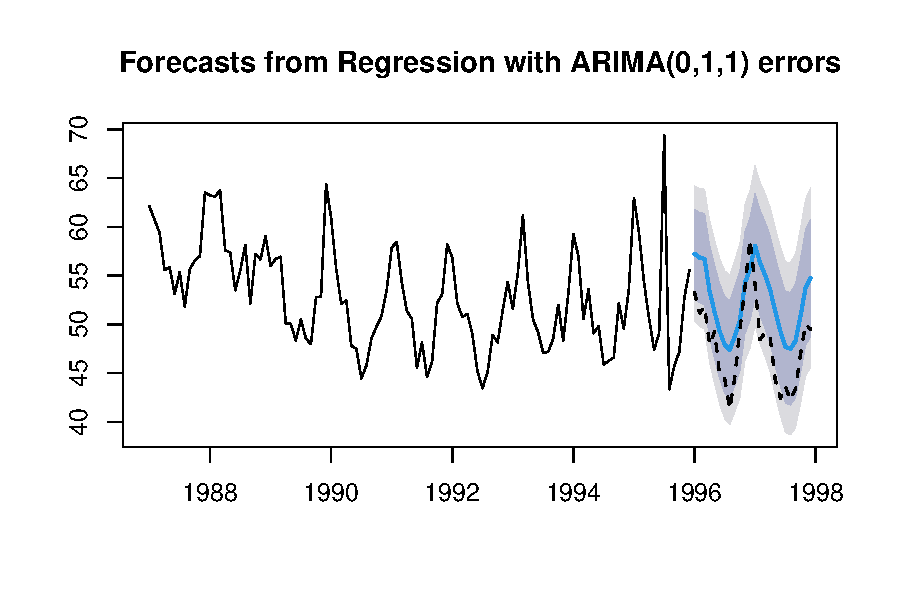
\includegraphics[width=0.65\linewidth]{images/arima-external-val}
    \caption{The prediction on validation dataset with ARIMA with external variables model}
    \label{arima-external-val}
\end{figure}

\vspace{4pt}
\subsection{Vector AR model}

In this section, we would like to implement Vector AR model. In order to avoid too many parameters (overfitting), we would like to control the lag.max=2. We run the 
following code to select the suitable lag order:
\begin{lstlisting}
VARselect(multi.training, lag.max=2, type="const")
\end{lstlisting}
The result is as follow:
\begin{lstlisting}
selection
AIC(n)  HQ(n)  SC(n) FPE(n) 
        2      2      1      2 

$criteria
                1           2
AIC(n)    10.83243    10.44461
HQ(n)     11.03611    10.81123
SC(n)     11.33496    11.34917
FPE(n) 50650.55661 34415.04660
\end{lstlisting}
Thus, we would like to use lag oder=2 in this vector AR model.
The fitted figure is as Figure \ref{arima-external-fit}. As we can see, the fitting seems very good, because there are 
$3+2\times 3^2=21$ parameters in this model, which means it is very possible to overfit.

\vspace{-15pt}
\begin{figure}[H]
    \centering
    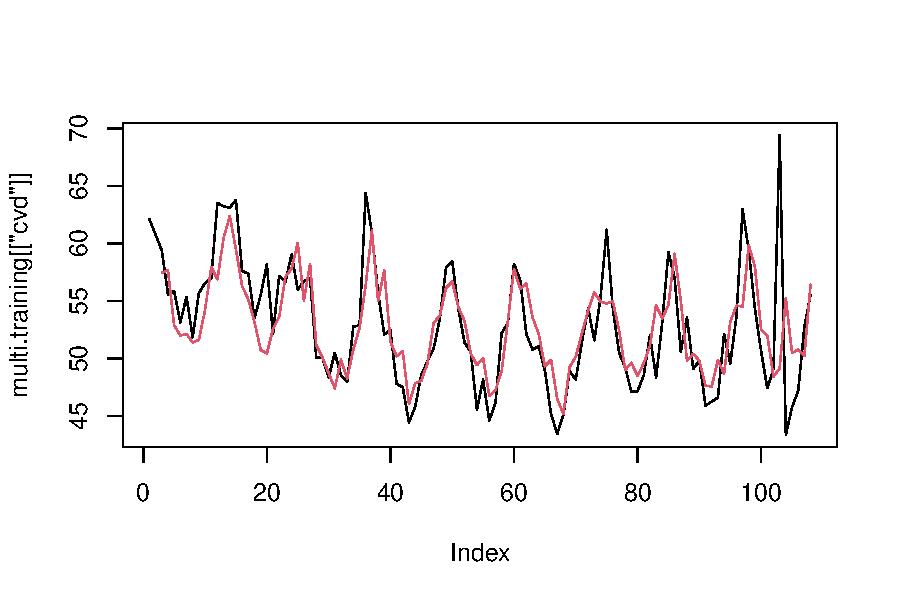
\includegraphics[width=0.65\linewidth]{images/var-fit}
    \caption{Vector AR model fitted figure}
    \label{var-fit}
\end{figure}
Then, we plot the residuals and the ACF figure of the residuals according to the the model result as Figure \ref{arima-external-acf}, which means we are going to check residuals of cvd.
\begin{figure}[H]
    \centering
    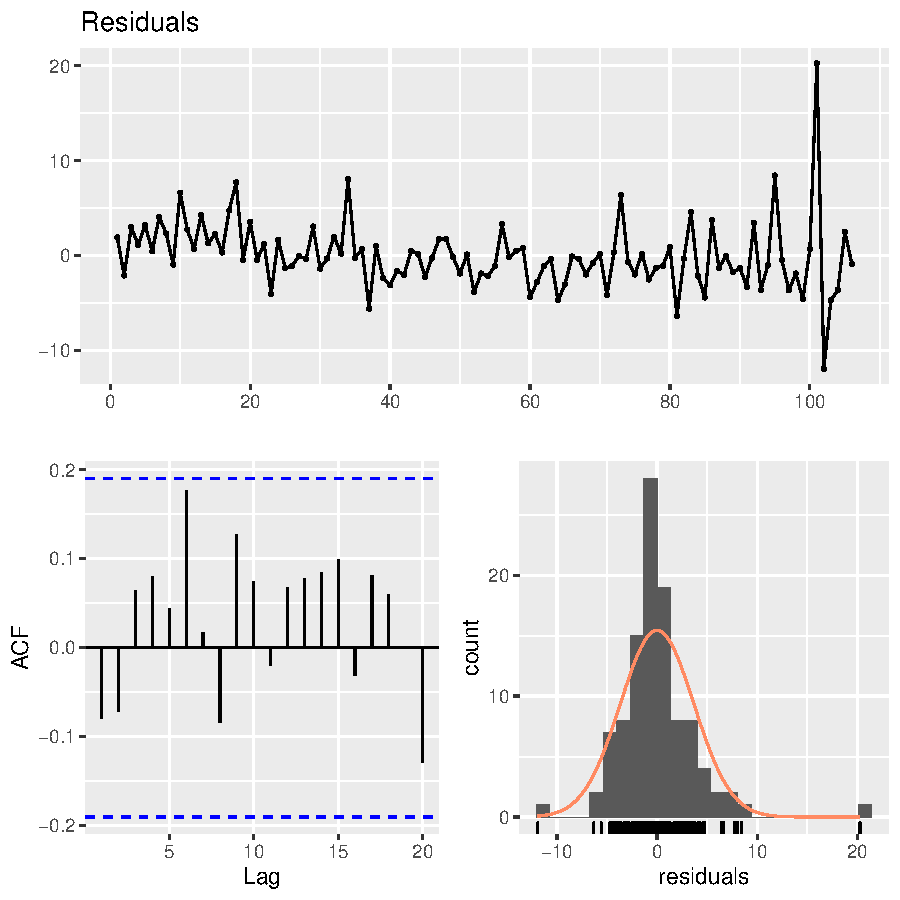
\includegraphics[width=0.58\linewidth]{images/var-acf}
    \caption{Check residuals of vector AR model}
    \label{var-acf}
\end{figure}
As we can see from Figure \ref{var-acf}, there is no significant acf, so that the model is somehow very good. 

\vspace{4pt}
Then, we would like to implement the fitted vector AR model on the validation dataset(1996.1-1997.12) in order to test the model's prediction accuracy. 
Firstly, we would like to see the fitted parameters as follow:
\begin{lstlisting}
VAR Estimation Results:
======================= 

Estimated coefficients for equation cvd: 
======================================== 
Call:
cvd = cvd.l1 + temp.l1 + pm10.l1 + o3.l1 + cvd.l2 + temp.l2 + 
        pm10.l2 + o3.l2 + const 

    cvd.l1     temp.l1     pm10.l1       o3.l1      cvd.l2     temp.l2  
    0.36411984 -0.29789871 -0.04243912  0.13608390  0.20698752  0.38811791 
    pm10.l2       o3.l2       const
    -0.01432600 -0.28986066 26.80201828 
\end{lstlisting}
Then, we can do forecast. As we can see in Figure \ref{var-forecast}, the dashed line is the true 
value of validation dataset, the blue line is the forcasted value of validation dataset. Then, we calculated the Root Mean Squard Error (RMSE) on the validation dataset. 
We can see that the RMSE is little larger, so that there might be overfitting in this model.

$\star$ RMSE = 5.67 $\star$
\begin{figure}[H]
    \centering
    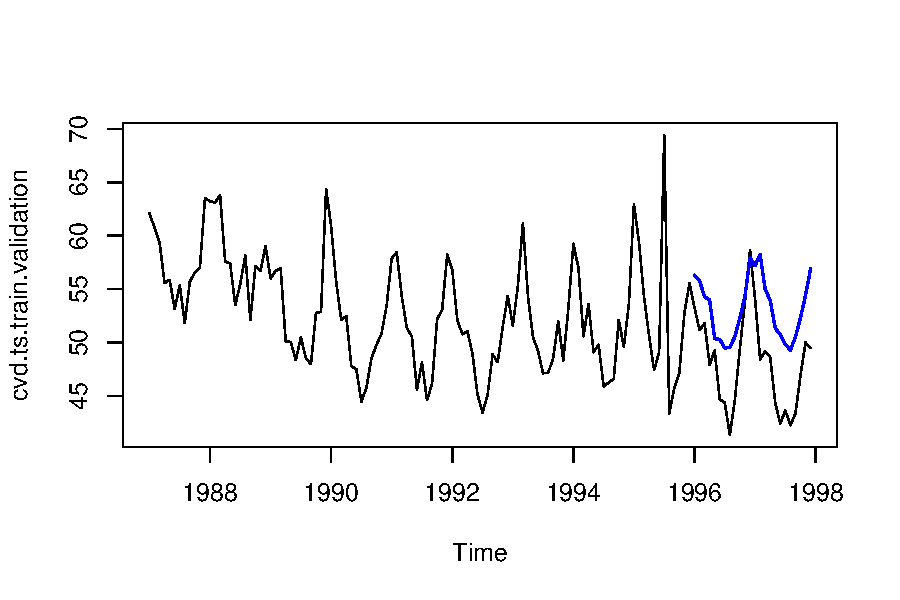
\includegraphics[width=0.58\linewidth]{images/var-forecast}
    \caption{Check residuals of vector AR model}
    \label{var-forecast}
\end{figure}

\vspace{4pt}
\subsection{Run the best model}

According to the RMSE value of the three models as follow (including the best univariate model-holt winters), we can find that the \textbf{ARIMA with external variables} is the bset. Thus, we would like to run ARIMA with external variables in the following.

\quad - Holt-winters:  RMSE = 5.08 

\quad - ARIMA with external variables:  RMSE = 3.16 $\star$

\quad - Vector AR: RMSE = 5.67

Firstly, we would like to run the best-performing model (ARIMA with external variables) on the 1987.1-1997.12 data (training dataset and validation dataset). 
We implement auto.arima to choose the parameters of 
"ARIMA with external variables" model.
\begin{lstlisting}
arima.external.best = auto.arima(cvd.ts.train.validation, 
        xreg=cbind(temp.ts.train.val, pm10.ts.train.val, o3.ts.train.val))
\end{lstlisting}
Then, we can see the result as follow
\begin{lstlisting}
Series: cvd.ts.train.validation 
Regression with ARIMA(0,1,2) errors 

Coefficients:
        ma1     ma2   drift  temp.ts.train.val  pm10.ts.train.val  o3.ts.train.val
    -0.7093 -0.1441 -0.0841          -0.3952             0.0411           0.0635
s.e. 0.0884  0.0914  0.0447           0.0498             0.0563           0.0663

sigma^2 estimated as 11.38:  log likelihood=-342.71
AIC=699.43   AICc=700.34   BIC=719.55
\end{lstlisting}
Thus, we get the parameters of ARIMA with external variables is:
the error $\eta_t$ is ARIMA(0,1,2). The fitted figure is as Figure \ref{arima-best-fit}.
\begin{figure}[H]
    \centering
    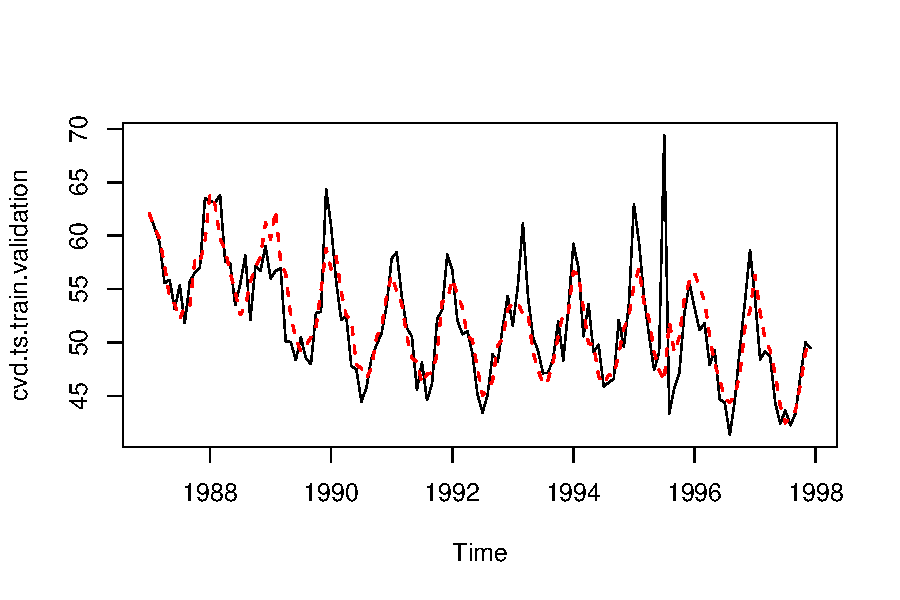
\includegraphics[width=0.65\linewidth]{images/arima-best-fit}
    \caption{AIRMA with external variables model fitted figure}
    \label{arima-best-fit}
\end{figure}
Then, we plot the residuals and the ACF figure of the residuals according to the the model result as Figure \ref{arima-best-acf}, which means we are going to check residuals. 
\begin{figure}[H]
    \centering
    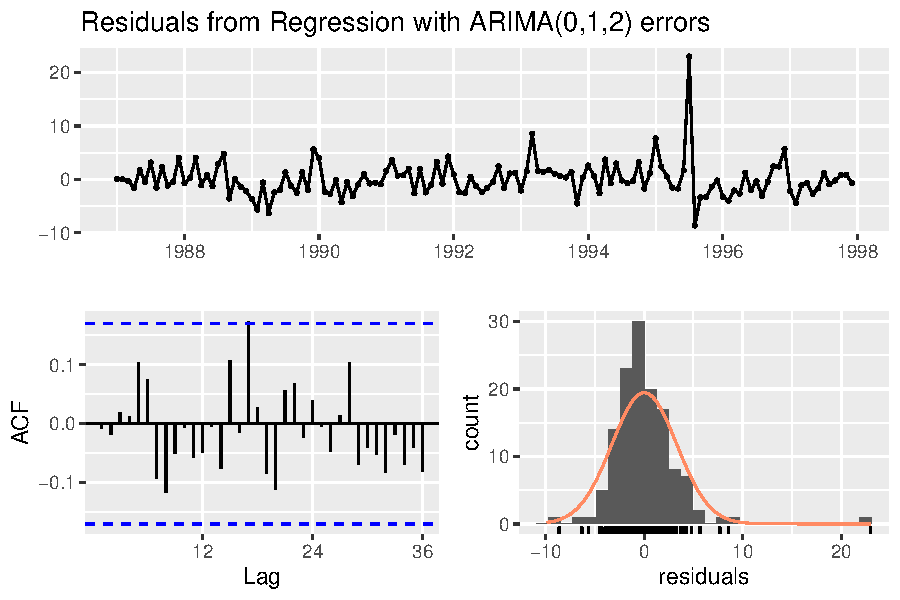
\includegraphics[width=0.65\linewidth]{images/arima-best-acf}
    \caption{Check residuals of ARIMA with external variables}
    \label{arima-best-acf}
\end{figure}
As we can see from Figure \ref{arima-best-acf},  
there is evident acf. Thus, we have to do Ljung-Box test of the residuals to see if the residuals exhibit serial correlation, the result is as follow:

\begin{lstlisting}
Ljung-Box test

data:  Residuals from Regression with ARIMA(0,1,2) errors
Q* = 18.836, df = 18, p-value = 0.402

Model df: 6.   Total lags used: 24
\end{lstlisting}
As we can see from the Ljung-Box test, the p-value equals 0.402, which is larger than 0.05, so that we should not reject the null hypothesis, which means 
the residuals does not exhibit serial correlation. Thus, we can believe that the ARIMA with external variables model is suitable.

\vspace{4pt}
Then, we would like to implement the fitted ARIMA with external variables model on the test dataset(1998.1-2000.12) in order to do forecast. As we can see in Figure \ref{arima-best-test}, the dashed line is the true 
value of test dataset, the blue line is the forcasted value of test dataset. Then, we calculated the Root Mean Squard Error (RMSE) on the test dataset. 

$\star$ RMSE = 3.42 $\star$
\begin{figure}[H]
    \centering
    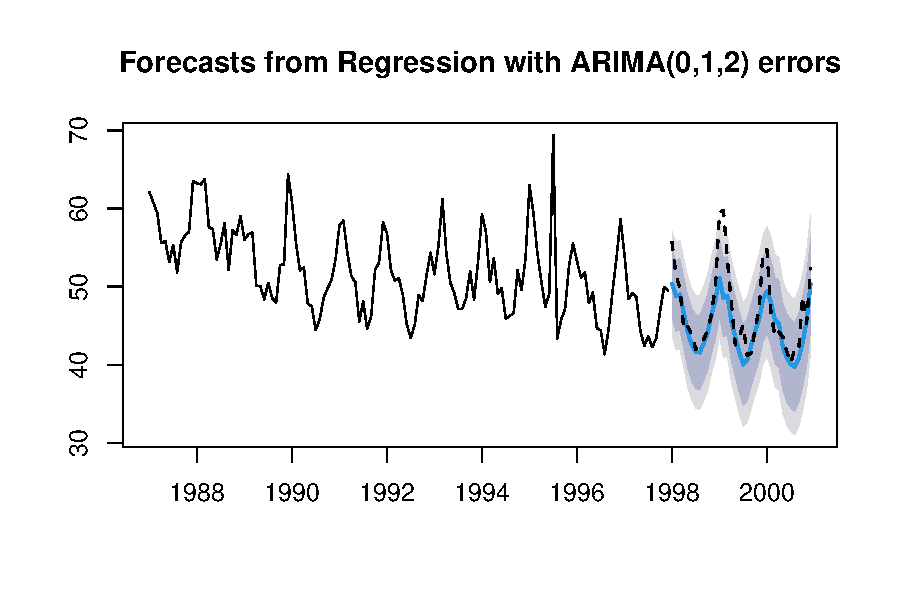
\includegraphics[width=0.65\linewidth]{images/arima-best-test}
    \caption{The prediction on test dataset with ARIMA with external variables model}
    \label{arima-best-test}
\end{figure}

\vspace{4pt}
\section{Conclusion}

After running the univariate and multivariate models, we finally find that the best model is ARIMA with external variables model, which is a multivariate model. 

\vspace{4pt}
The conclusion makes sense bacause we know that the cardiovascular death should be correlated with the temperature (temp) and pollution (pm10 and o3). Thus, the result is better when we consider the 
external variables. Above all, the model is good to predict the number of ardiovascular death.
\end{document}

